% -*- coding: utf-8 -*-

\documentclass{beamer}
\mode<presentation>
{
% \usetheme{Boadilla}
% \usetheme{Malmoe}

% \usetheme{Warsaw}
% \setbeamercovered{transparent}

\setbeamertemplate{background canvas}[vertical shading][bottom=white,top=structure.fg!25]
\usetheme{Warsaw}
\setbeamertemplate{headline}{}
\setbeamertemplate{footline}{}
% \setbeamersize{text margin left=0.5cm}


}

\usepackage[french]{babel}
\usepackage[utf8]{inputenc}

\usepackage{times}
\usepackage[T1]{fontenc}

\usepackage{multimedia}

\title[Analyse de la répartition de CAS et WAP]{Analyse de la répartition des gènes CAS et WAP dans les noyaux de cellules HC11}
% \subtitle{Include Only If Paper Has a Subtitle}

\author{Ga\"etan Lehmann}
\institute[INRA]{INRA, Biologie du Développement et de la Reproduction}
\date[Club chromatine - 18/10/2007]{Club chromatine - 18 octobre 2007}
% \subject{Theoretical Computer Science}

% \pgfdeclareimage[height=0.5cm]{university-logo}{university-logo-filename}
% \logo{\pgfuseimage{university-logo}}

% \AtBeginSection[]
% {
%   \begin{frame}<beamer>
%     \frametitle{Plan}
%     \tableofcontents[currentsection,currentsubsection]
%   \end{frame}
% }

\AtBeginSubsection[]
{
  \begin{frame}<beamer>
    \frametitle{Plan}
    \tableofcontents[currentsection,currentsubsection]
  \end{frame}
}

\begin{document}

\frame
{
  \titlepage
  \begin{center}
    {\small En collaboration avec} Maria Ballester {\small et} Kiên Kiêu
  \end{center}
}

\frame
{
  \frametitle{Plan}
  \tableofcontents % [pausesections]
}
  
\section{Introduction}

  \frame
  {
    \frametitle{Les images}
    \begin{itemize}
    \item Trois canaux (noyaux, CAS et WAP) \\
        \uncover<1->
        {
          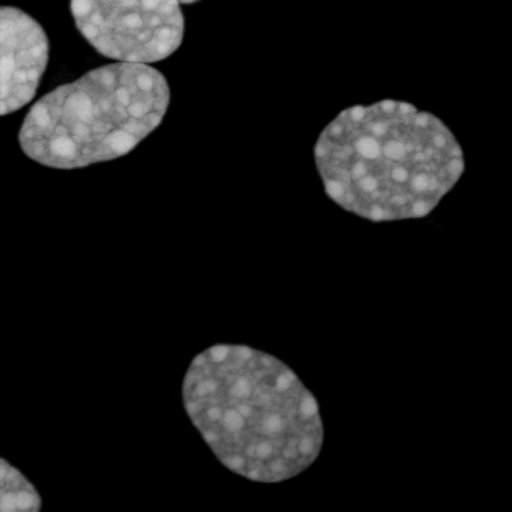
\includegraphics[height=3cm]{noyaux.png}~
          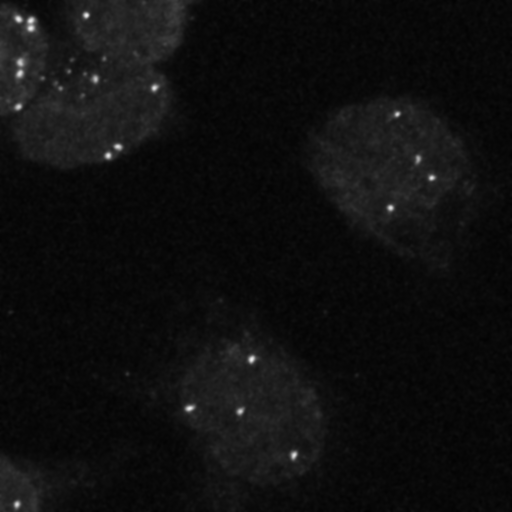
\includegraphics[height=3cm]{cas-gauss.png}~
          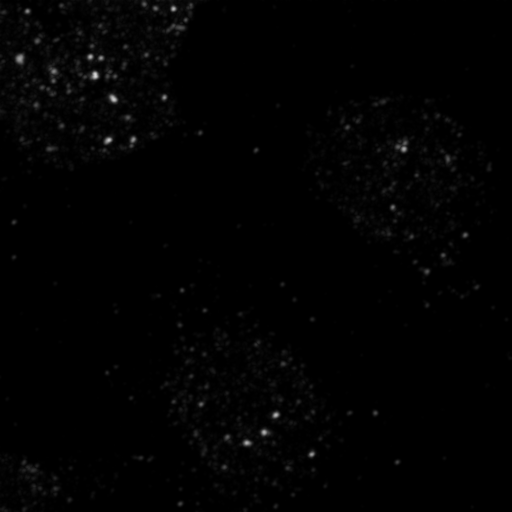
\includegraphics[height=3cm]{wap-gauss.png} \\
        }
        Les images contiennent les informations nécessaires pour l'analyse de la répartition. \\
        \uncover<4->{{\em Une procédure pour chaque type d'image.}}
      \item<2-> En trois dimensions
        \begin{itemize}
          \item Mieux adaptées que les images en 2D.
          \item Difficile à manipuler et à visualiser... Automatisation ?
        \end{itemize}
      \item<3-> En grand nombre \\
        {\em Automatisation}
    \end{itemize}
  }
    
  
\section{Analyse d'image}
  
  \subsection{Débruitage}
    
    \frame
    {
      \frametitle{Débruitage des images de microscopie confocale}
      \begin{itemize}
        \item<2-> Filtre médian
        \item<3-> Filtre gaussien
      \end{itemize}
      \begin{center}
        \only<1>{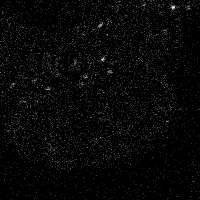
\includegraphics[height=6cm]{denoising-native.png}}
        \only<2>{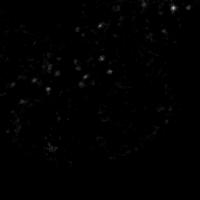
\includegraphics[height=6cm]{denoising-median.png}}
        \only<3>{
\includegraphics[height=6cm]{denoising-gaussian.png}}
      \end{center}
    }
    
  \subsection{Segmentation des noyaux}
    
    \frame
    {
      \frametitle{Seuillage, histogramme unimodale et gradient}
      \begin{center}
        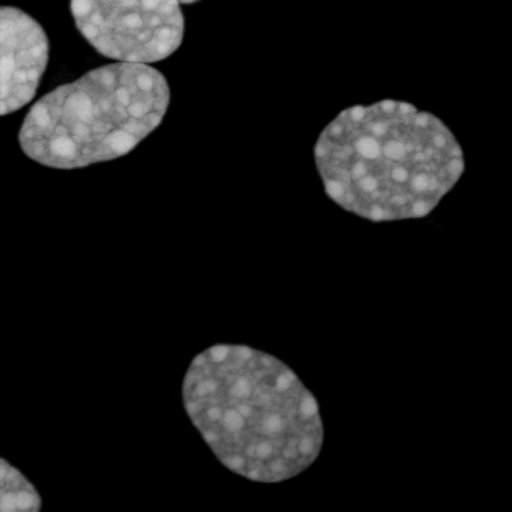
\includegraphics[height=3.8cm]{noyaux.png}~
        \only<2>{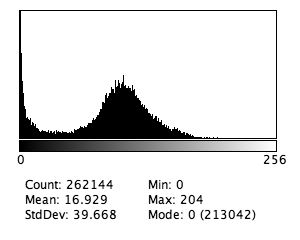
\includegraphics[height=3.8cm]{noyaux-histo2D.png}}\only<3->{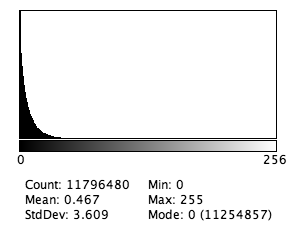
\includegraphics[height=3.8cm]{noyaux-histo.png}}\\ 
        \uncover<4->{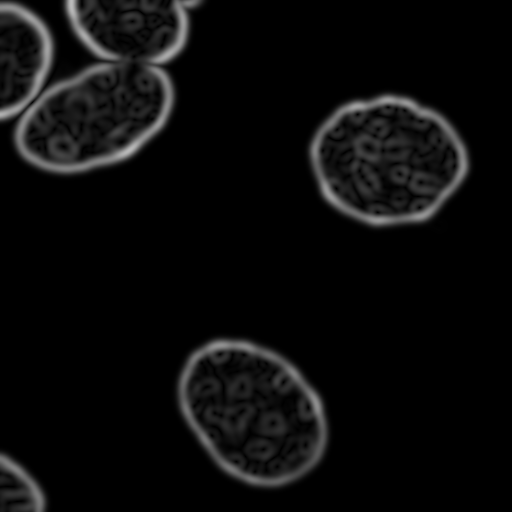
\includegraphics[height=3.8cm]{noyaux-gradient.png}}
        ~\uncover<5->{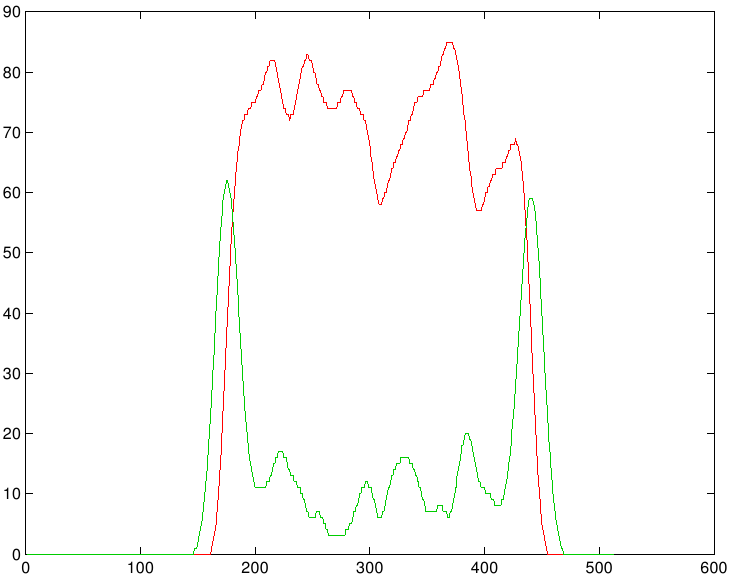
\includegraphics[height=3.75cm]{profile-gradient.png}}
       \end{center}
   }

    \frame
    {
      \frametitle{Robust Automatic Threshold Selection}
      \begin{itemize}
        \item<1->{Le seuil est la moyenne des intensités dans l'image des noyaux pondérée par le gradient.}
        $$
        Th = \frac{\sum\limits_{p~\in~D}G(p)~.~I(p)}{\sum\limits_{p~\in~D}G(p)}
        $$
%        $$
%        T = \frac{\sum\limits_{p~\in~D}G(p)\only<2->{\alert<2>{^m}}~.~I(p)}{\sum\limits_{p~\in~D}G(p)\only<2->{\alert<2>{^m}}}
%        $$
%        \item<2->{Utilisation d'une puissance du gradient pour diminuer la sensibilité au bruit (en général, $m = 2$).}
%        \item<3->{Suppression des petites zones qui perturbent le calcul :}
%          \begin{itemize}
%            \item avec une ouverture par attribut pour les zone claires,
%            \item avec un {\em fill hole} pour les zone sombres.
%          \end{itemize}
%        \item<4->{Le masque binaire produit devra être amélioré.}    
      \end{itemize}
      \begin{center}
        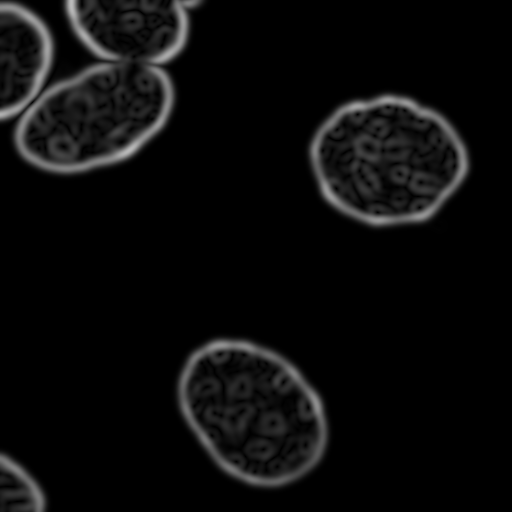
\includegraphics[height=3.8cm]{noyaux-gradient.png}
        ~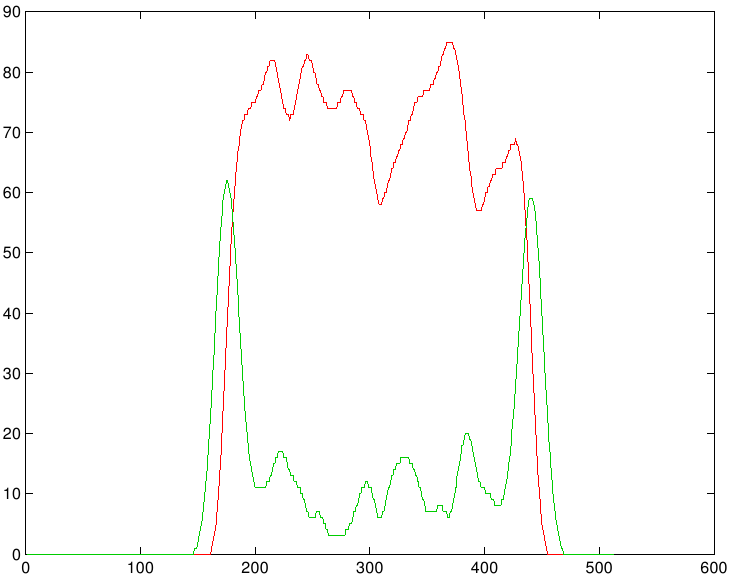
\includegraphics[height=3.75cm]{profile-gradient.png}
      \end{center}
    }
  
    \frame
    {
      \frametitle{La segmentation du noyaux, en image et pas à pas}
      \begin{center}
        \only<1>{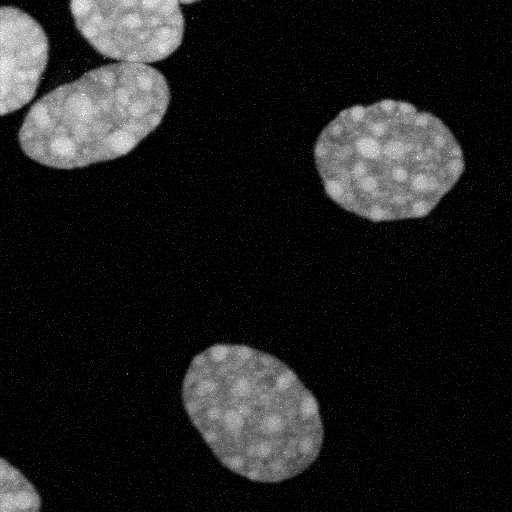
\includegraphics[height=6cm]{noyaux-noisy.png}\\L'image des noyaux}
        \only<2>{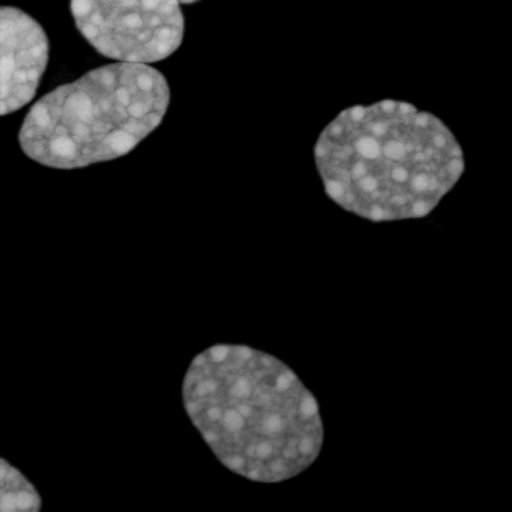
\includegraphics[height=6cm]{noyaux.png}\\Débruitage}
        \only<3>{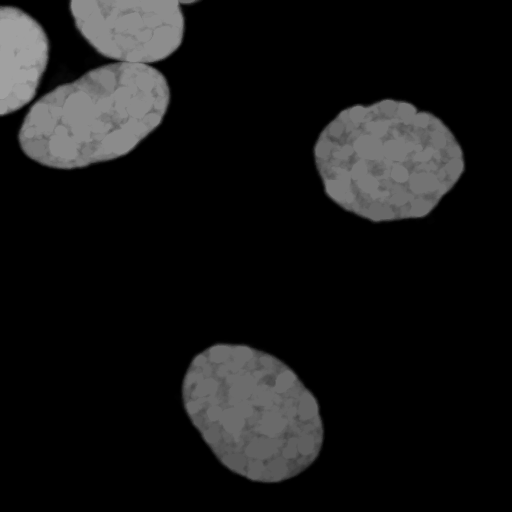
\includegraphics[height=6cm]{noyaux-open.png}\\Suppression des petites zones claires}
        \only<4>{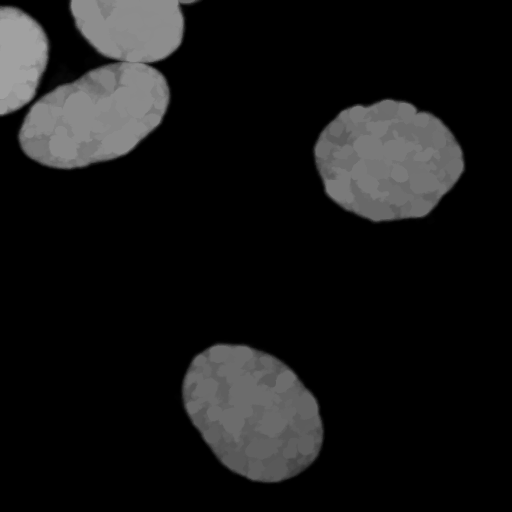
\includegraphics[height=6cm]{noyaux-fill.png}\\Remplissage des petites zones sombres}
        \only<5-6>{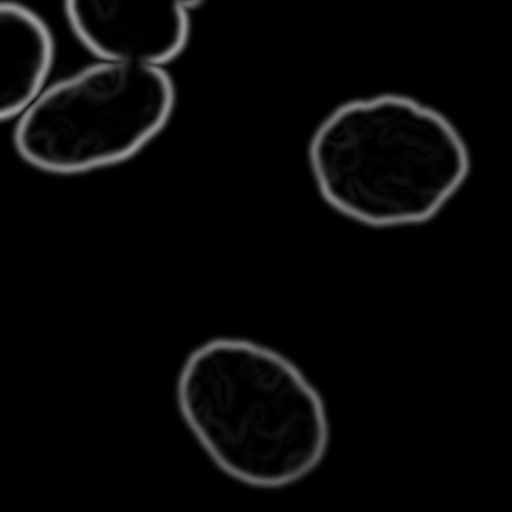
\includegraphics[height=6cm]{noyaux-gradient2.png}}\only<6>{~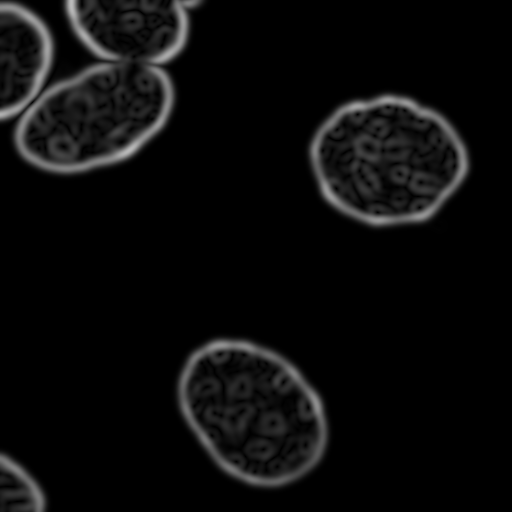
\includegraphics[height=6cm]{noyaux-gradient.png}}\only<5-6>{\\Gradient}
        \only<7>{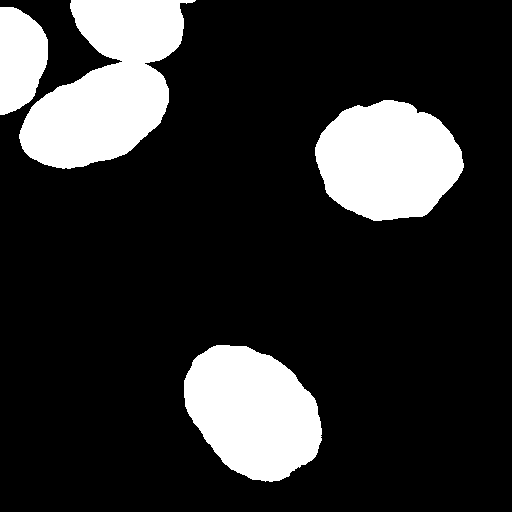
\includegraphics[height=6cm]{noyaux-rats.png}\\Seuillage}
        \only<8>{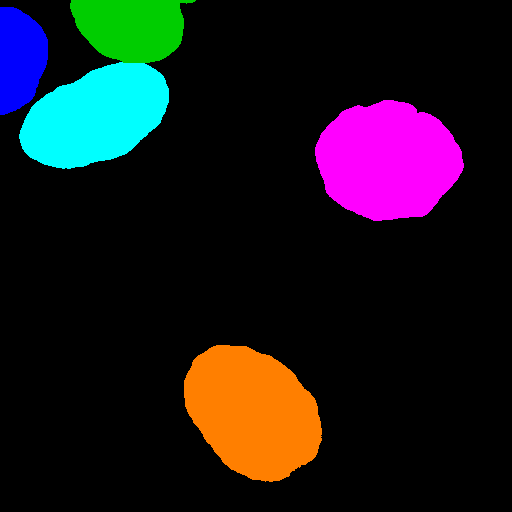
\includegraphics[height=6cm]{noyaux-ws.png}\\Séparation des noyaux et labellisation par watershed}
        \only<9>{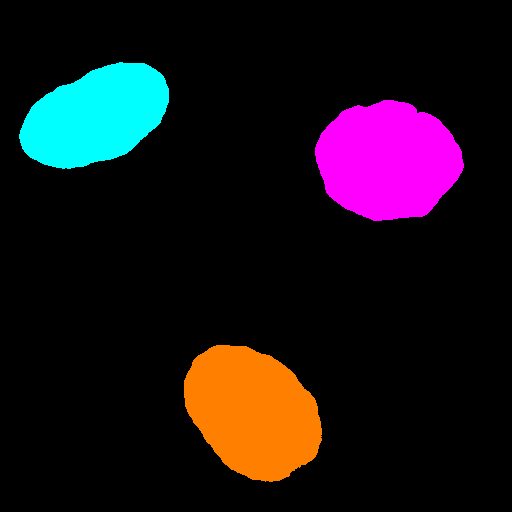
\includegraphics[height=6cm]{noyaux-border.png}\\Suppression des objets sur le bord}
%     \end{center} 
%    }
%    
%    \frame
%    {
%      \begin{center}
%        \frametitle{Validation visuelle}
        \only<10>{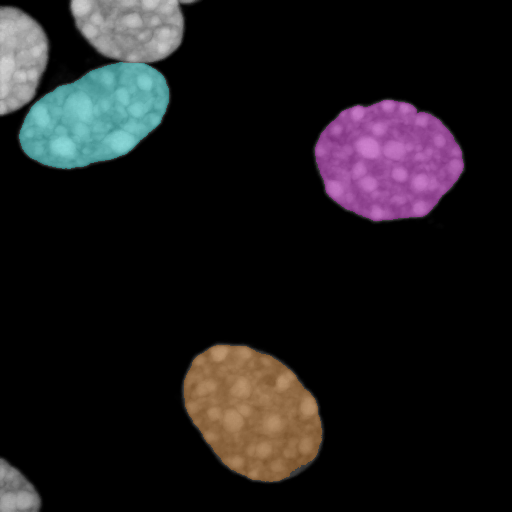
\includegraphics[height=6cm]{noyaux-overlay.png}\\Superposition de l'image de départ et de la segmentation}
     \end{center} 
    }
    
  
  \subsection{Segmentation des spots de CAS}
    
    \frame
    {
      \frametitle{Tophat par attribut}
      \begin{itemize}
        \item Bon contraste entre le fond et les spots.
        \item Fond {\em parfois} de niveau élevé et texturé.
      \end{itemize}
      \begin{center}
        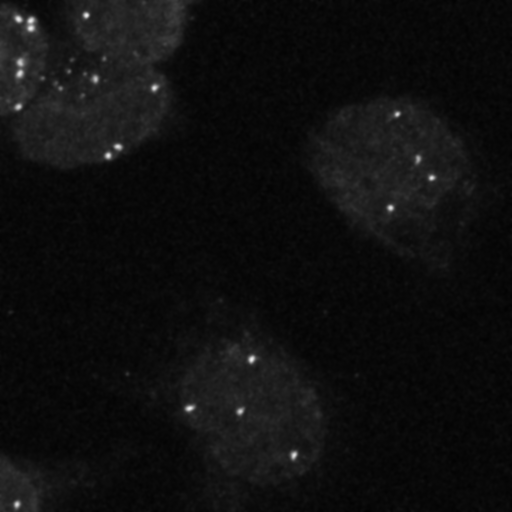
\includegraphics[height=5cm]{cas-gauss.png}
      \end{center}
      \uncover<2->{Suppression du fond en éliminant les objets trop grands suivie d'un seuillage.}
    }
    
    \frame
    {
      \frametitle{La segmentation des gènes CAS en image}
      \begin{center}
        \only<1>{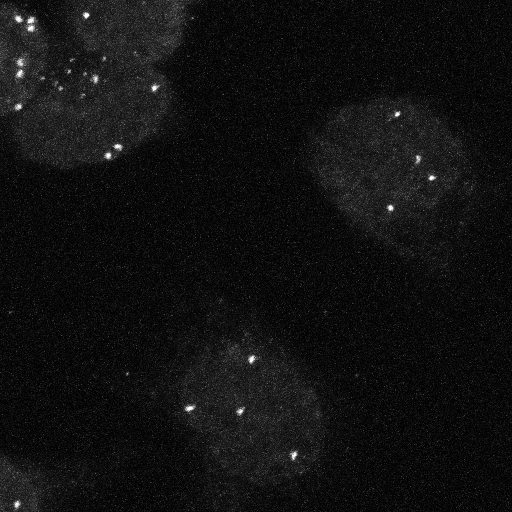
\includegraphics[height=6cm]{cas-noisy.png}\\L'image brute}
        \only<2>{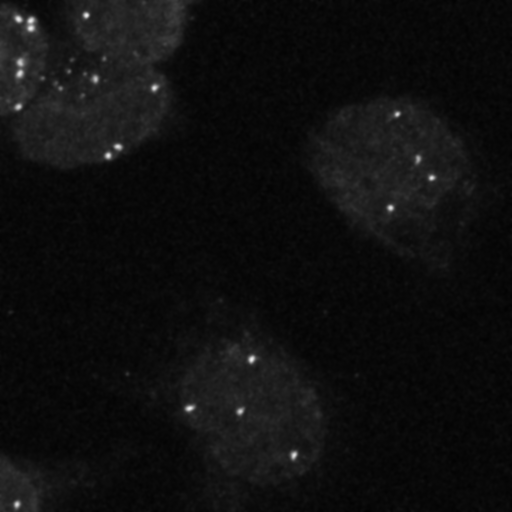
\includegraphics[height=6cm]{cas-gauss.png}\\Débruitage}
        \only<3>{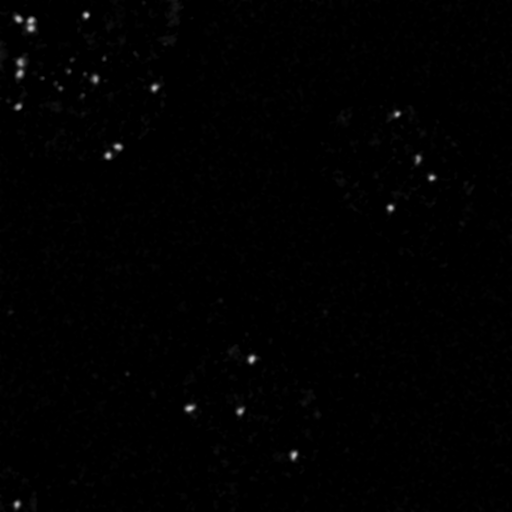
\includegraphics[height=6cm]{cas-tophat.png}\\Tophat par attribut}
        \only<4>{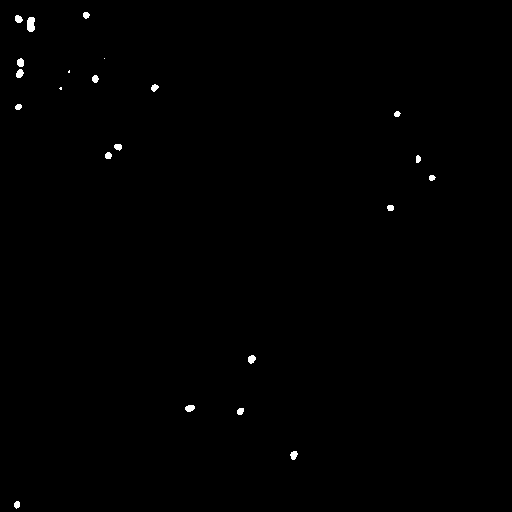
\includegraphics[height=6cm]{cas-th.png}\\Seuillage}
        \only<5>{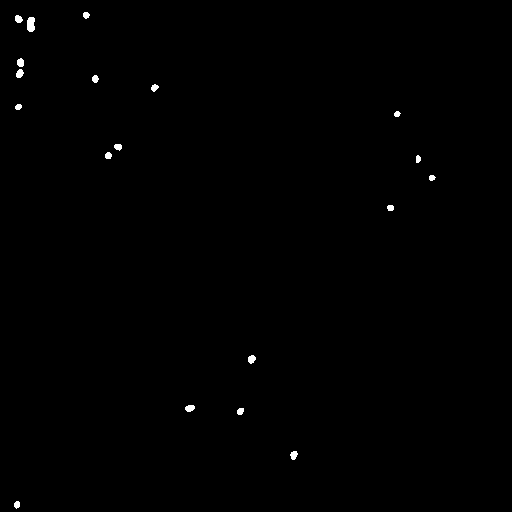
\includegraphics[height=6cm]{cas-binopen.png}\\Suppression des objets trop petits}
        \only<6>{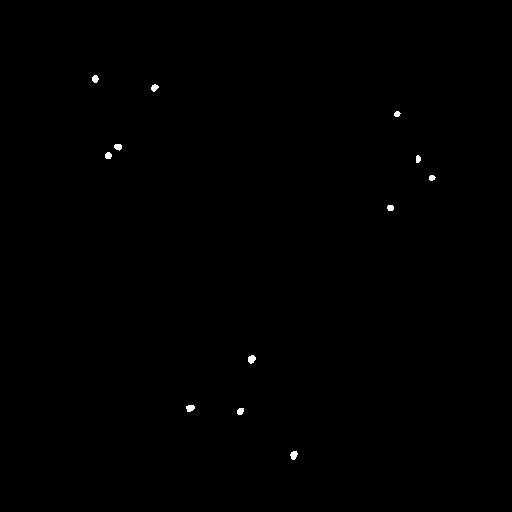
\includegraphics[height=6cm]{cas-mask.png}\\Masquage}
        \only<7>{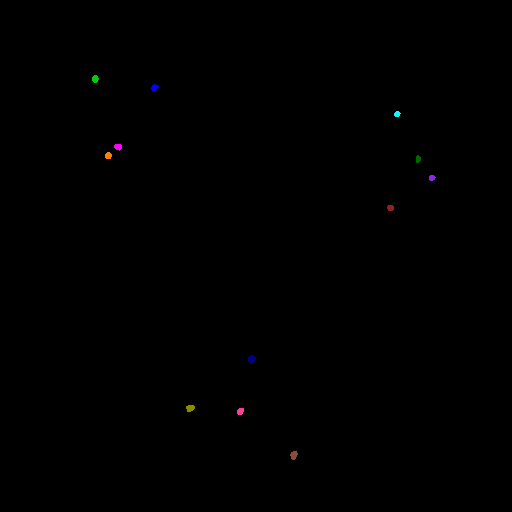
\includegraphics[height=6cm]{cas-color.png}\\Labellisation}
%     \end{center} 
%    }
%    
%    \frame
%    {
%      \begin{center}
%        \frametitle{Validation visuelle}
        \only<8>{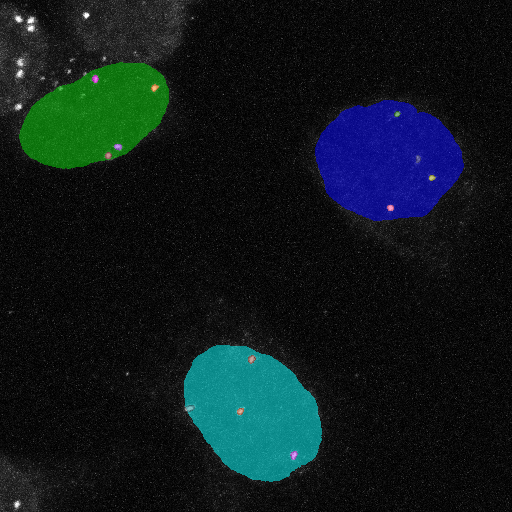
\includegraphics[height=6cm]{cas-overlay.png}\\Superposition de l'image de départ, de la segmentation des gènes CAS et de la segmentation des noyaux.}
     \end{center} 
    }
    
    
    
  \subsection{Segmentation des spots de WAP}
    
    \frame
    {
      \frametitle{Garder les quatres pics les plus importants}
      \begin{itemize}
        \item Contraste faible entre le fond et les spots.
      \end{itemize}
      \begin{center}
        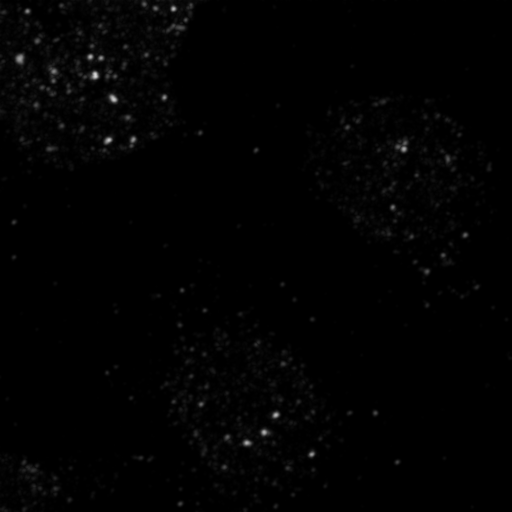
\includegraphics[height=5cm]{wap-gauss.png}
      \end{center}
      \uncover<2->{Conserver seulement les quatres spots les plus importants.}
    }
  
    \frame
    {
      \frametitle{Volume levelling}
      Quel critère utiliser pour déterminer les pics importants ?
      \begin{itemize}
        \item<1-> l'intensité
        \item<1-> le contraste (différence d'intensité avec le fond)
        \item<2-> la taille (le nombre de pixels dans le spot)
        \item<3-> la somme des intensités
        \item<3-> \alert<4>{le contraste * la taille : « volume levelling »}
      \end{itemize}
    }
  
    \frame
    {
      \frametitle{La segmentation des gènes WAP en image}
      \begin{center}
        \only<1>{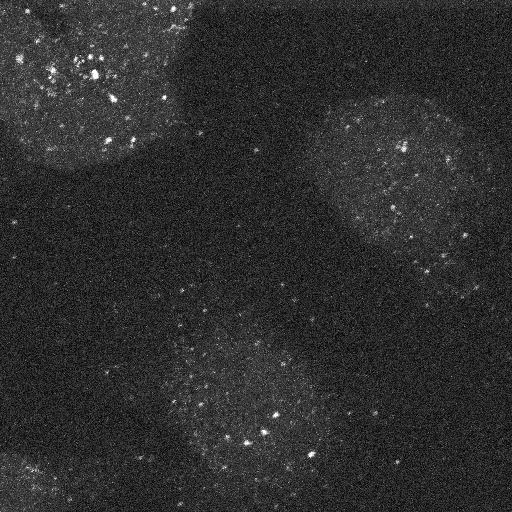
\includegraphics[height=6cm]{wap-noisy.png}\\L'image brute}
        \only<2>{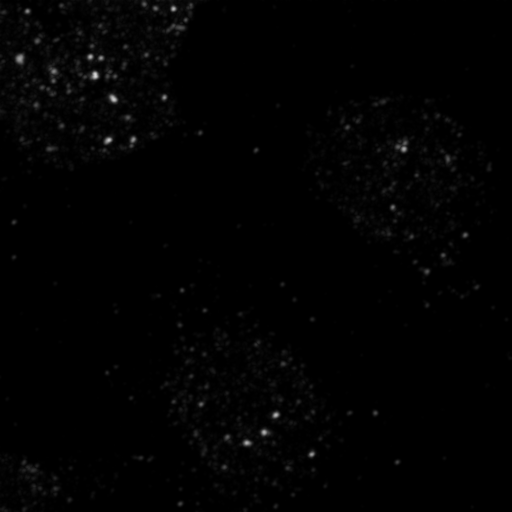
\includegraphics[height=6cm]{wap-gauss.png}\\Débruitage}
        \only<3>{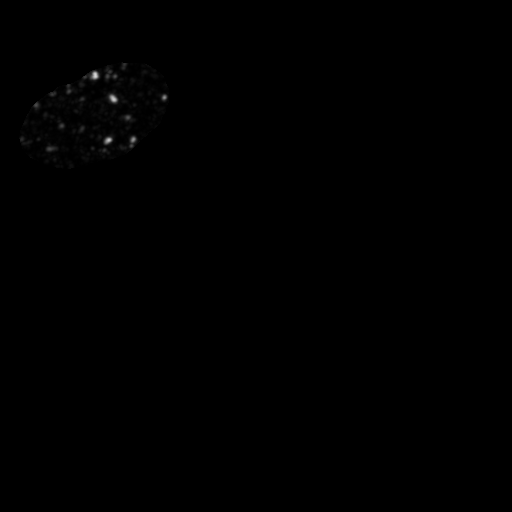
\includegraphics[height=6cm]{wap-mask.png}\\Masquage du noyau}
        \only<4>{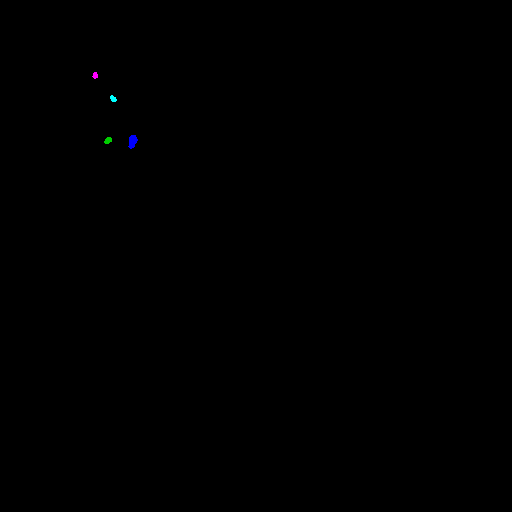
\includegraphics[height=6cm]{wap-color.png}\\Extraction des quatre spots les plus importants}
%     \end{center} 
%    }
%    
%    \frame
%    {
%      \frametitle{Validation visuelle}
%      \begin{center}
        \only<5>{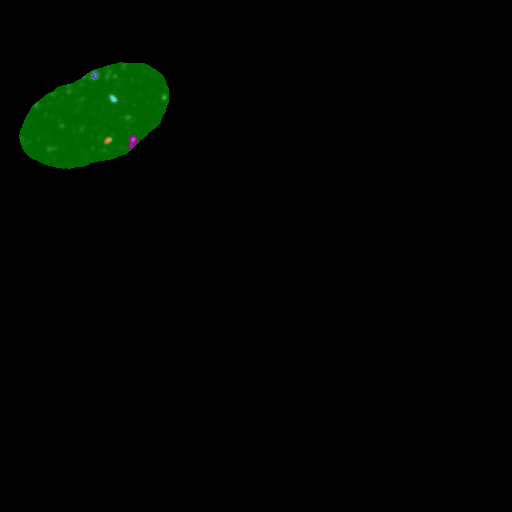
\includegraphics[height=6cm]{wap-overlay.png}\\Superposition de l'image de départ, de la segmentation des gènes WAP et de la segmentation des noyaux.}
     \end{center} 
    }
    
    \frame
    {
      \frametitle{Cycle de validation et d'amélioration}
      \begin{itemize}
        \item<1-> Définition des éléments à repérer dans les images
        \item<2-> Mise en place de la procédure de segmentation
        \item<2-> Production d'une petite série d'image segmentée
        \item<3-> Correction par l'expert biologiste (Maria)
        \item<4-> Amélioration de la procédure de segmentation
        \item<4-> Utilisation de la procédure de segmentation sur la totalité des images
        \item<5-> Correction par l'expert biologiste (Maria)
      \end{itemize}
    }
    
\section{Mesures}
    
  \subsection{Position des gènes}
    
    \frame
    {
      \frametitle{Mesure de la position des gènes}
      \begin{itemize}
        \item<1-> La position du gène est estimée en calculant la position moyenne des pixels dans le spot pondérée par l'intensité des pixels.
        \item<2-> Précision supérieure à la résolution de l'image
      \end{itemize}
      \begin{center}
        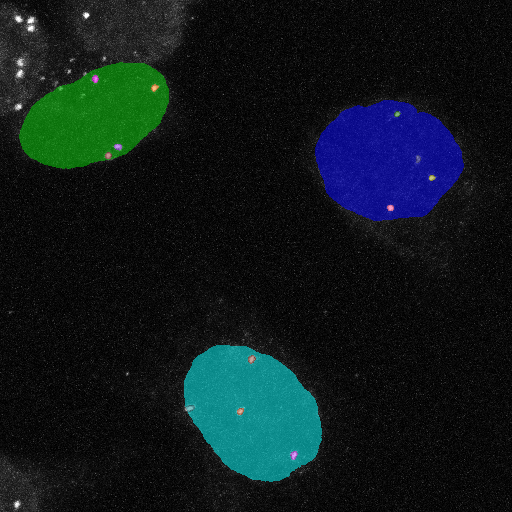
\includegraphics[height=5cm]{cas-overlay.png}
      \end{center} 
    }
    
  \subsection{Fraction de volume érodé}
    
    \frame
    {
      \frametitle{Fraction de volume érodé}
      \begin{center}
        \only<1>{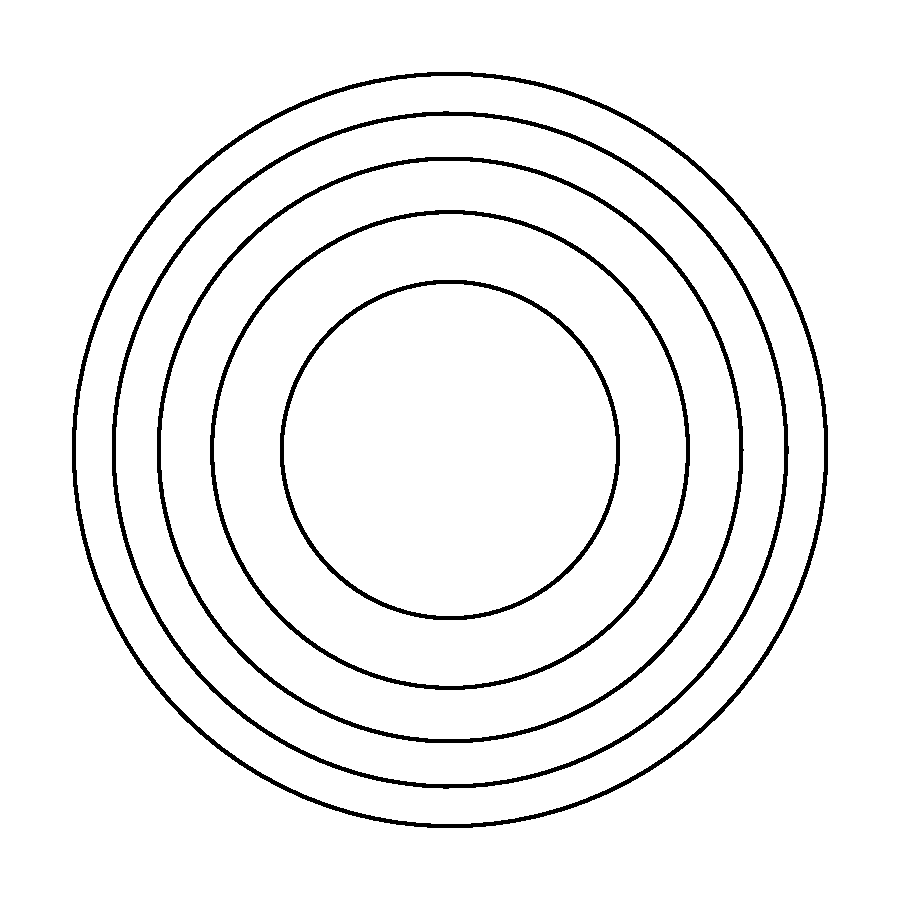
\includegraphics[height=6cm]{expose_12062007-plot-shells.pdf}}
        \only<2>{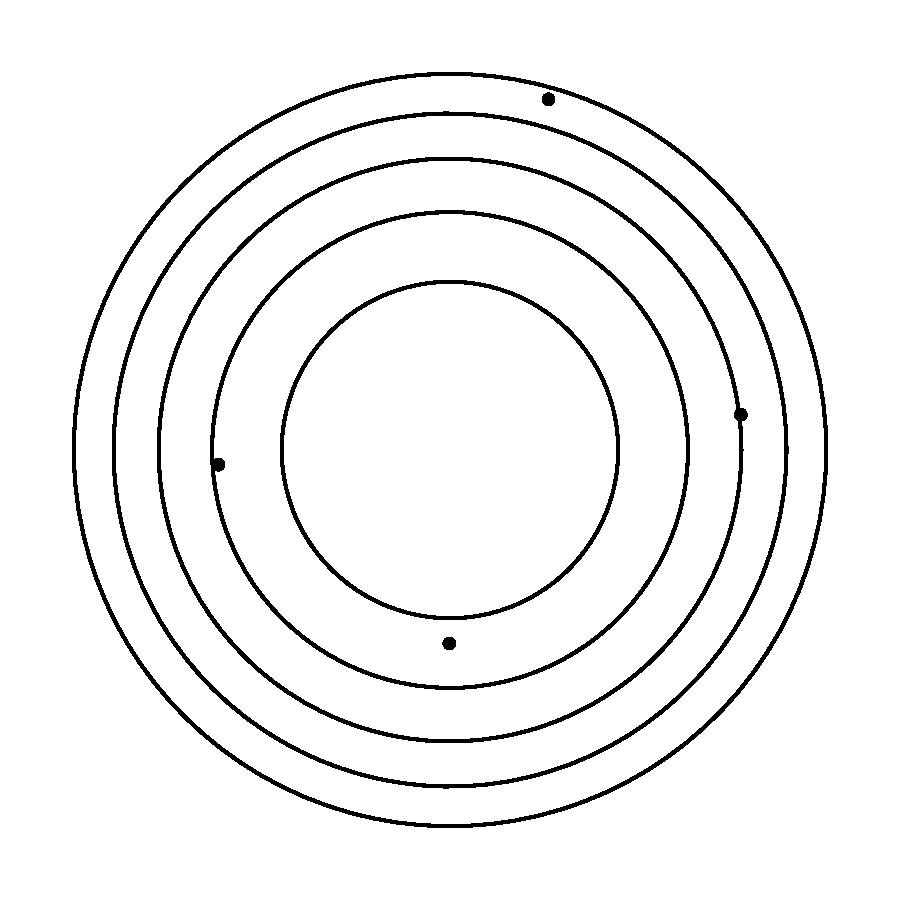
\includegraphics[height=6cm]{expose_12062007-003.pdf}}
        \only<3>{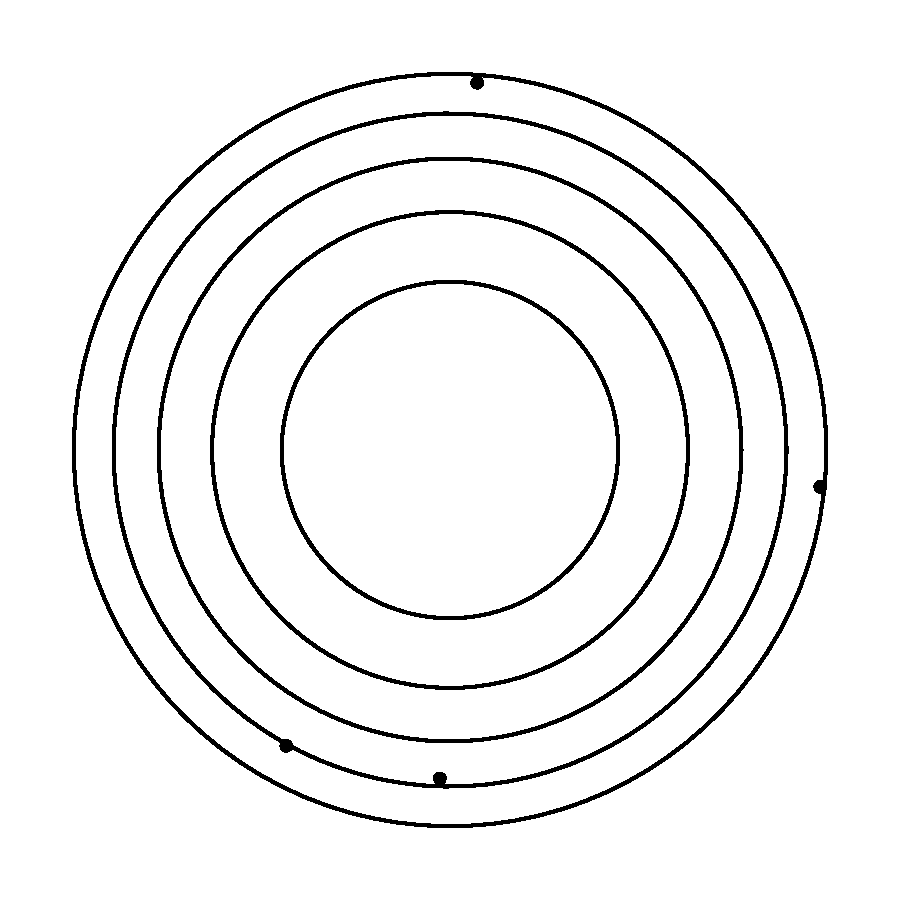
\includegraphics[height=6cm]{expose_12062007-004.pdf}}
        \only<4>{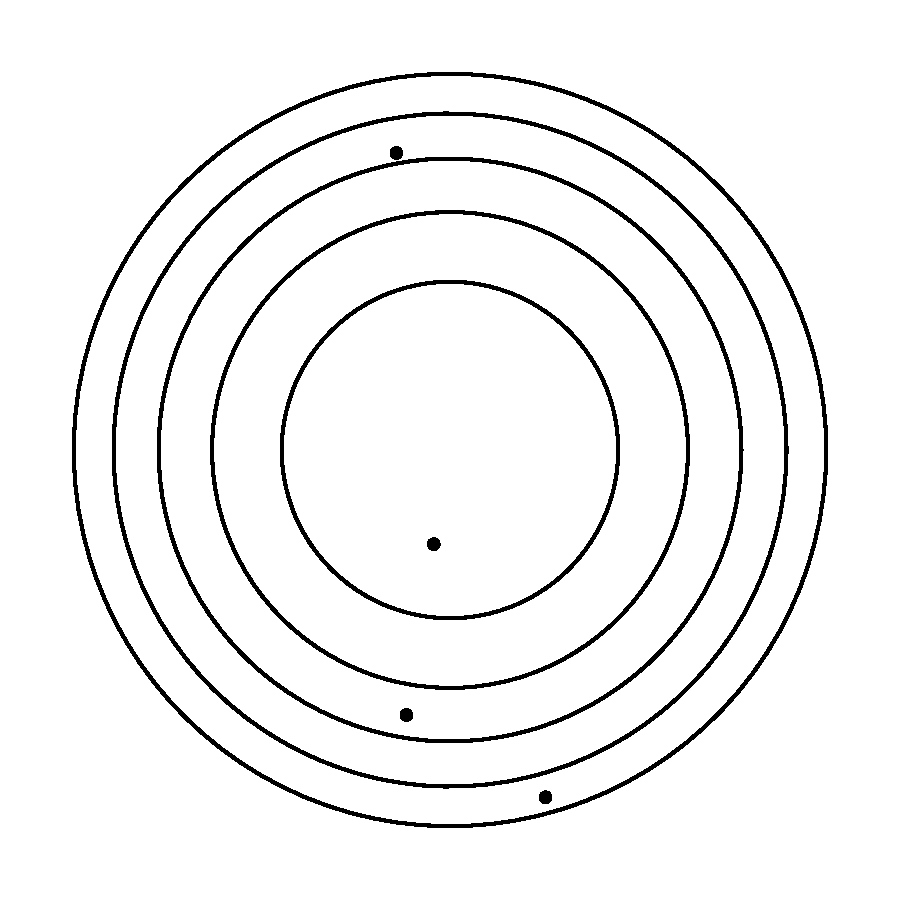
\includegraphics[height=6cm]{expose_12062007-005.pdf}}
        \only<5>{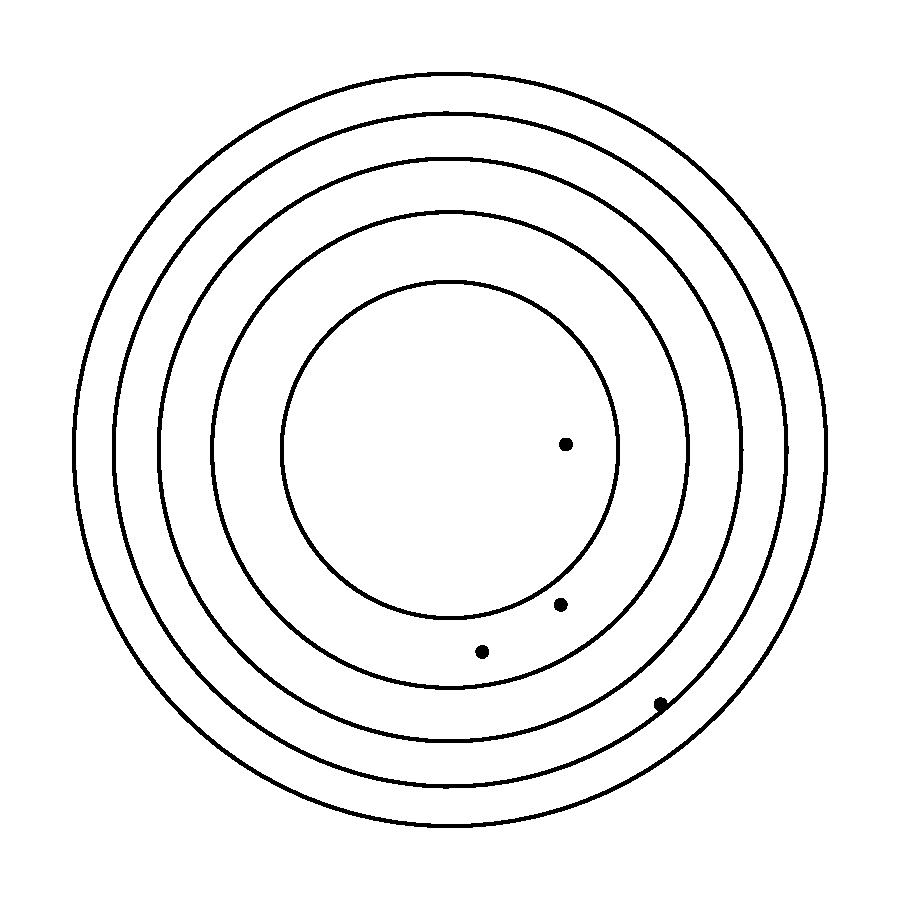
\includegraphics[height=6cm]{expose_12062007-006.pdf}}
        \only<6-7>{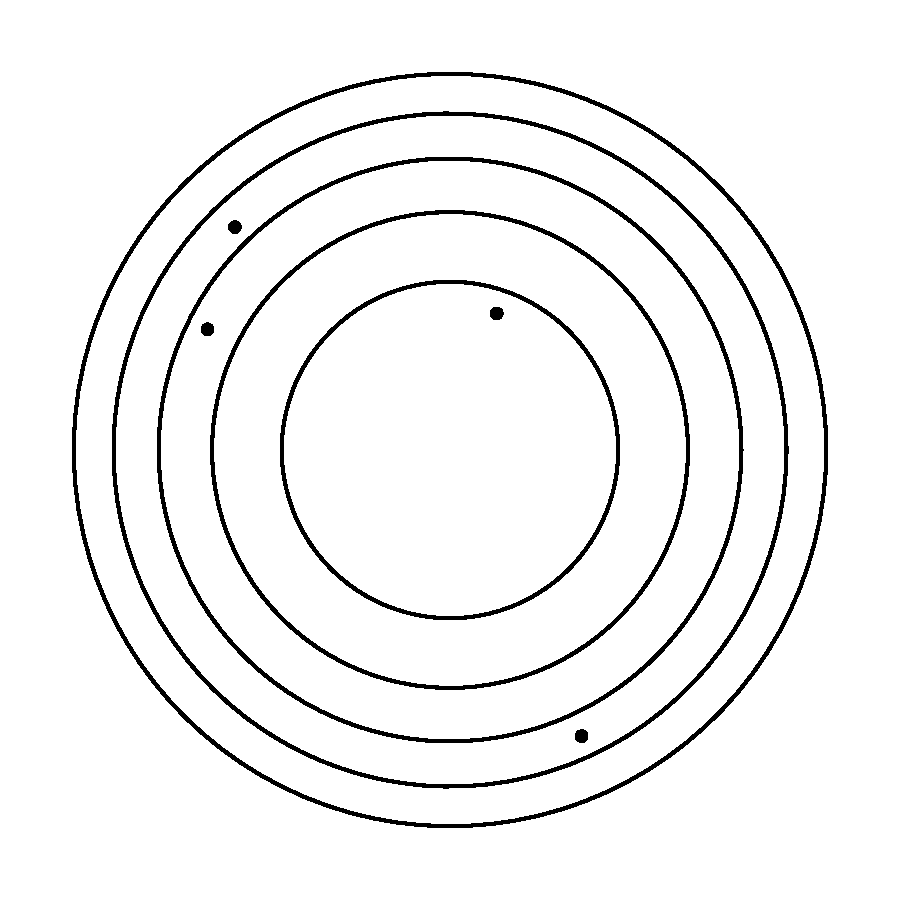
\includegraphics[height=6cm]{expose_12062007-plot-last-pattern.pdf}}
        \only<7>{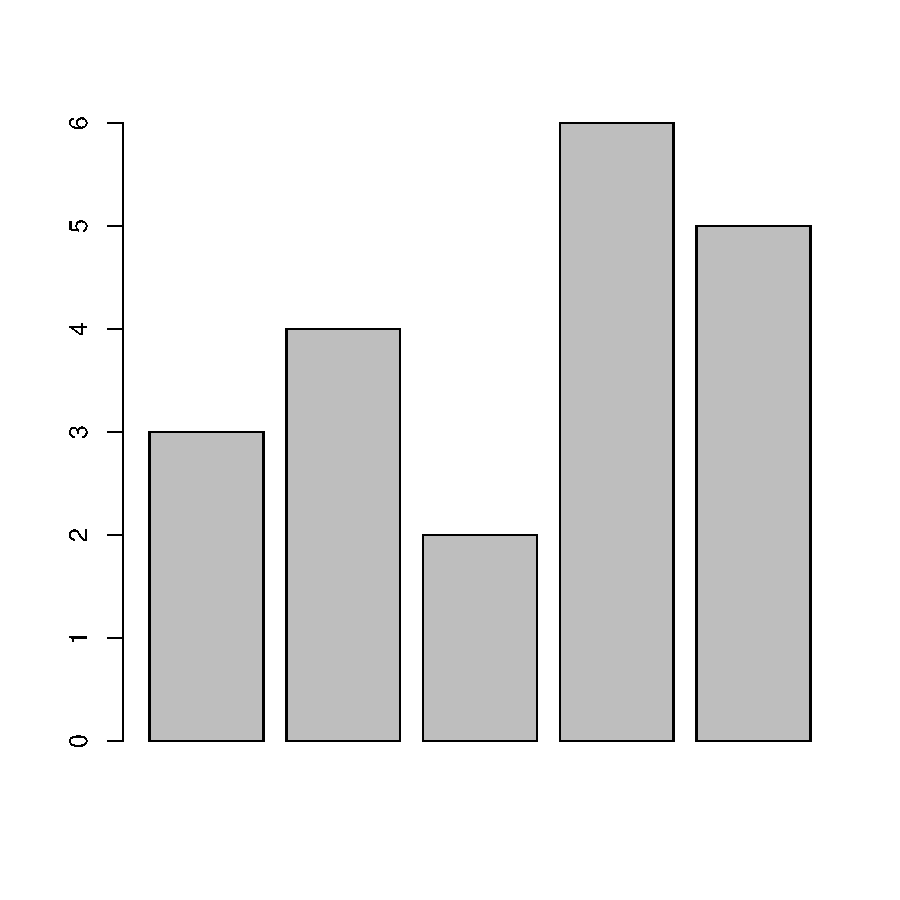
\includegraphics[height=6cm]{expose_12062007-009.pdf}}
        \only<8->{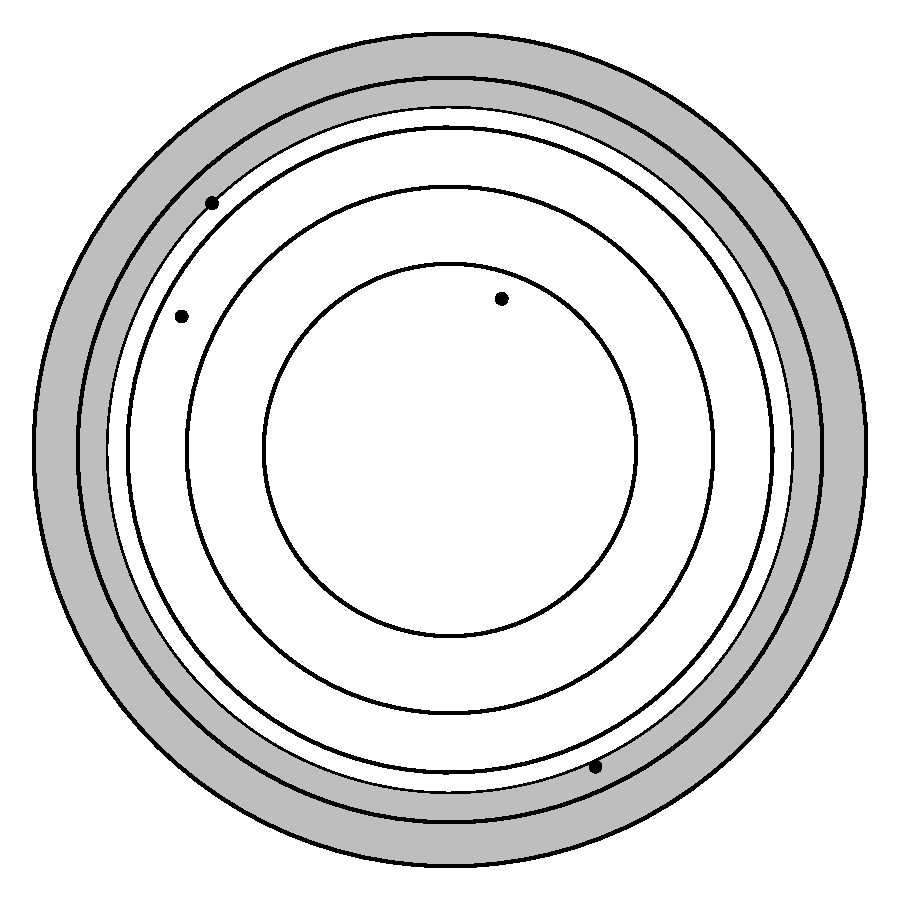
\includegraphics[height=6cm]{expose_12062007-008.pdf}}
        \\
        \uncover<9->{fve = fraction du volume plus proche de la membrane nucléaire que le gène}
      \end{center}
    }
  
    \frame
    {
      \frametitle{Mesure de la fraction de volume érodé}
      \begin{center}
        \only<1>{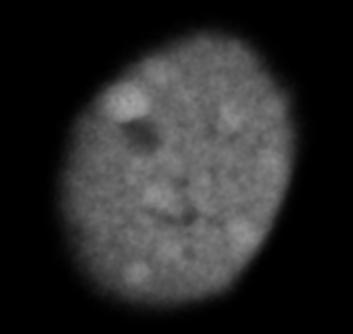
\includegraphics[height=6cm]{20070320_20_z16_smooth.jpg}\\Le noyau}
        \only<2>{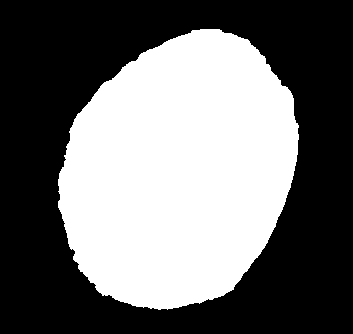
\includegraphics[height=6cm]{bin.png}\\Le masque du noyau}
        \only<3>{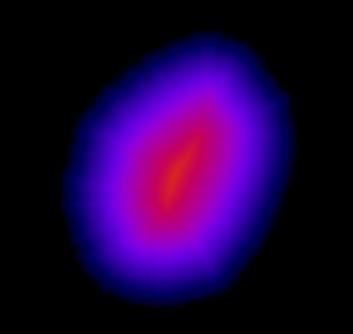
\includegraphics[height=6cm]{dist-col.jpg}\\La carte de distance}
        \only<4>{\includegraphics[height=6cm]{dist-col-dot.jpg}\\La carte de distance}
        \only<5>{\includegraphics[height=6cm]{dist-col-dot-level.jpg}\\Les lignes de niveau}
      \end{center} 
    }
    
%  \subsection{Distance à la membrane}
%    
%    \frame
%    {
%      \frametitle{Mesure de la distance à la membrane}
%      Lecture directe dans la carte de distance.
%      \begin{center}
%        \includegraphics[height=6cm]{dist-col-dot.jpg}
%      \end{center} 
%    }
    
%  \subsection{Mesure de l'applatissement}
%    
%    \frame
%    {
%      \frametitle{Applatissement}
%    }
    
\section{Analyse statistique}
  
  \frame
  {
    \frametitle{Plan}
    \tableofcontents[currentsection,currentsubsection]
  }
  
  \frame
  {
    \frametitle{Analyse statistique}
    \begin{itemize}
%      \item Intégrer les données issues de l'analyse d'image
%      \item Étudier l'influence de différents facteurs sur la FVE
%      \item Produire des résultats ayant un sens biologique
      
      \item Utilisation de méthodes d'analyse classiques
        \begin{itemize}
          \item représentations graphiques
          \item modèles linéaires gaussiens
          \item test du khi-deux)
        \end{itemize}
      \item Recherche de facteurs (autres que la stimulation hormonale) qui peuvent avoir des effets sur la répartition spatiale des gènes.
    \end{itemize}
  }
  
\begin{frame}[fragile] 
\frametitle{Exemple de sortie} 
\small \begin{verbatim} 
Call:
lm(formula = evf ~ (gene + stimulation + slide)^2,
   data = gene)

Residuals:
     Min       1Q   Median       3Q      Max 
-0.68230 -0.14844 -0.00975  0.13609  0.71883 

Coefficients:
             Estimate Std. Error t value Pr(>|t|)    
(Intercept)  4.579e-01  8.989e-03  50.938  < 2e-16 ***
csn         -2.230e-01  8.972e-03 -24.857  < 2e-16 ***
stim         1.479e-02  1.174e-02   1.259  0.20822    
slide1       1.299e-05  8.989e-03   0.001  0.99885    
csn:stim     3.356e-02  1.163e-02   2.886  0.00396 ** 
csn:slide1  -1.388e-03  5.785e-03  -0.240  0.81049    
stim:slide1 -9.109e-03  1.174e-02  -0.776  0.43810    
\end{verbatim} \normalsize
\end{frame} 
  
\section*{Conclusion}

  \frame
  {
    \frametitle{Fin}
    \begin{center}
      \includegraphics[height=3.37cm]{cas-overlay.png}~
      \includegraphics[height=3.37cm]{expose_12062007-008.pdf} \\
      \includegraphics[height=3.37cm]{expose_12062007-009.pdf}~
      \movie[width=3.37cm,height=3cm,poster,loop,autostart]{}{vrmaria.avi} % ,externalviewer,showcontrols
    \end{center}
  }
  
\end{document}
